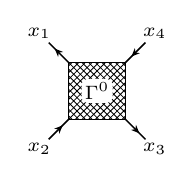
\begin{tikzpicture}[x=0.600cm, y=0.600cm, line width=0.550pt, baseline={([yshift=-0.6ex]0,0)}]
  \draw (0.000,0.000) -- (-0.600,0.600);
  \draw (0.000,0.000) -- (-0.600,-0.600);
  \draw (0.000,0.000) -- (0.600,-0.600);
  \draw (0.000,0.000) -- (0.600,0.600);
  \draw (-0.600,0.600) -- (-1.024,1.024);
  \fill (-0.896,0.896) -- (-0.824,0.717) -- (-0.811,0.811) -- (-0.717,0.824) -- cycle;
  \draw (-0.600,-0.600) -- (-1.024,-1.024);
  \fill (-0.728,-0.728) -- (-0.907,-0.800) -- (-0.813,-0.813) -- (-0.800,-0.907) -- cycle;
  \draw (0.600,-0.600) -- (1.024,-1.024);
  \fill (0.896,-0.896) -- (0.824,-0.717) -- (0.811,-0.811) -- (0.717,-0.824) -- cycle;
  \draw (0.600,0.600) -- (1.024,1.024);
  \fill (0.728,0.728) -- (0.907,0.800) -- (0.813,0.813) -- (0.800,0.907) -- cycle;
  \fill[white] (-0.600,-0.600) rectangle (0.600,0.600);
  \draw[line width=0.303pt] (-0.600,0.531) -- (-0.531,0.600) (-0.600,0.390) -- (-0.390,0.600) (-0.600,0.249) -- (-0.249,0.600) (-0.600,0.107) -- (-0.107,0.600) (-0.600,-0.034) -- (0.034,0.600) (-0.600,-0.176) -- (0.176,0.600) (-0.600,-0.317) -- (0.317,0.600) (-0.600,-0.459) -- (0.459,0.600) (-0.600,-0.600) -- (0.600,0.600) (-0.459,-0.600) -- (0.600,0.459) (-0.317,-0.600) -- (0.600,0.317) (-0.176,-0.600) -- (0.600,0.176) (-0.034,-0.600) -- (0.600,0.034) (0.107,-0.600) -- (0.600,-0.107) (0.249,-0.600) -- (0.600,-0.249) (0.390,-0.600) -- (0.600,-0.390) (0.531,-0.600) -- (0.600,-0.531) (-0.600,-0.531) -- (-0.531,-0.600) (-0.600,-0.390) -- (-0.390,-0.600) (-0.600,-0.249) -- (-0.249,-0.600) (-0.600,-0.107) -- (-0.107,-0.600) (-0.600,0.034) -- (0.034,-0.600) (-0.600,0.176) -- (0.176,-0.600) (-0.600,0.317) -- (0.317,-0.600) (-0.600,0.459) -- (0.459,-0.600) (-0.600,0.600) -- (0.600,-0.600) (-0.459,0.600) -- (0.600,-0.459) (-0.317,0.600) -- (0.600,-0.317) (-0.176,0.600) -- (0.600,-0.176) (-0.034,0.600) -- (0.600,-0.034) (0.107,0.600) -- (0.600,0.107) (0.249,0.600) -- (0.600,0.249) (0.390,0.600) -- (0.600,0.390) (0.531,0.600) -- (0.600,0.531);
  \begin{scope}
  \clip (-0.600,-0.600) rectangle (0.600,0.600);
  \node[font=\scriptsize, inner sep=1.2pt, fill=white, rounded corners=2pt] at (0.000,0.000) {$\Gamma^0$};
  \end{scope}
  \draw (-0.600,-0.600) rectangle (0.600,0.600);
  \node[font=\scriptsize, inner sep=0pt, anchor=315] at (-1.088,1.088) {$x_{1}$};
  \node[font=\scriptsize, inner sep=0pt, anchor=45] at (-1.088,-1.088) {$x_{2}$};
  \node[font=\scriptsize, inner sep=0pt, anchor=135] at (1.088,-1.088) {$x_{3}$};
  \node[font=\scriptsize, inner sep=0pt, anchor=225] at (1.088,1.088) {$x_{4}$};
\end{tikzpicture}
\allowbreak\;{+}\; 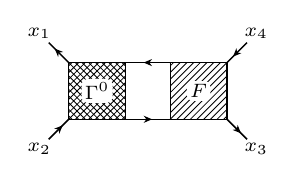
\begin{tikzpicture}[x=0.600cm, y=0.600cm, line width=0.550pt, baseline={([yshift=-0.6ex]0,0)}]
  \draw (-0.475,-0.600) -- (0.475,-0.600);
  \fill (0.089,-0.600) -- (-0.089,-0.524) -- (-0.031,-0.600) -- (-0.089,-0.676) -- cycle;
  \draw (0.475,0.600) -- (-0.475,0.600);
  \fill (-0.089,0.600) -- (0.089,0.524) -- (0.031,0.600) -- (0.089,0.676) -- cycle;
  \draw (1.075,0.000) -- (0.475,0.600);
  \draw (1.075,0.000) -- (0.475,-0.600);
  \draw (1.075,0.000) -- (1.675,-0.600);
  \draw (1.075,0.000) -- (1.675,0.600);
  \draw (-1.075,0.000) -- (-1.675,0.600);
  \draw (-1.075,0.000) -- (-1.675,-0.600);
  \draw (-1.075,0.000) -- (-0.475,-0.600);
  \draw (-1.075,0.000) -- (-0.475,0.600);
  \draw (-1.675,0.600) -- (-2.099,1.024);
  \fill (-1.971,0.896) -- (-1.899,0.717) -- (-1.886,0.811) -- (-1.792,0.824) -- cycle;
  \draw (-1.675,-0.600) -- (-2.099,-1.024);
  \fill (-1.803,-0.728) -- (-1.982,-0.800) -- (-1.888,-0.813) -- (-1.875,-0.907) -- cycle;
  \draw (1.675,-0.600) -- (2.099,-1.024);
  \fill (1.971,-0.896) -- (1.899,-0.717) -- (1.886,-0.811) -- (1.792,-0.824) -- cycle;
  \draw (1.675,0.600) -- (2.099,1.024);
  \fill (1.803,0.728) -- (1.982,0.800) -- (1.888,0.813) -- (1.875,0.907) -- cycle;
  \fill[white] (0.475,-0.600) rectangle (1.675,0.600);
  \draw[line width=0.303pt] (0.475,0.531) -- (0.544,0.600) (0.475,0.390) -- (0.685,0.600) (0.475,0.249) -- (0.826,0.600) (0.475,0.107) -- (0.968,0.600) (0.475,-0.034) -- (1.109,0.600) (0.475,-0.176) -- (1.251,0.600) (0.475,-0.317) -- (1.392,0.600) (0.475,-0.459) -- (1.534,0.600) (0.475,-0.600) -- (1.675,0.600) (0.616,-0.600) -- (1.675,0.459) (0.758,-0.600) -- (1.675,0.317) (0.899,-0.600) -- (1.675,0.176) (1.041,-0.600) -- (1.675,0.034) (1.182,-0.600) -- (1.675,-0.107) (1.324,-0.600) -- (1.675,-0.249) (1.465,-0.600) -- (1.675,-0.390) (1.606,-0.600) -- (1.675,-0.531);
  \begin{scope}
  \clip (0.475,-0.600) rectangle (1.675,0.600);
  \node[font=\scriptsize, inner sep=1.2pt, fill=white, rounded corners=2pt] at (1.075,0.000) {$F$};
  \end{scope}
  \draw (0.475,-0.600) rectangle (1.675,0.600);
  \fill[white] (-1.675,-0.600) rectangle (-0.475,0.600);
  \draw[line width=0.303pt] (-1.675,0.531) -- (-1.606,0.600) (-1.675,0.390) -- (-1.465,0.600) (-1.675,0.249) -- (-1.324,0.600) (-1.675,0.107) -- (-1.182,0.600) (-1.675,-0.034) -- (-1.041,0.600) (-1.675,-0.176) -- (-0.899,0.600) (-1.675,-0.317) -- (-0.758,0.600) (-1.675,-0.459) -- (-0.616,0.600) (-1.675,-0.600) -- (-0.475,0.600) (-1.534,-0.600) -- (-0.475,0.459) (-1.392,-0.600) -- (-0.475,0.317) (-1.251,-0.600) -- (-0.475,0.176) (-1.109,-0.600) -- (-0.475,0.034) (-0.968,-0.600) -- (-0.475,-0.107) (-0.826,-0.600) -- (-0.475,-0.249) (-0.685,-0.600) -- (-0.475,-0.390) (-0.544,-0.600) -- (-0.475,-0.531) (-1.675,-0.531) -- (-1.606,-0.600) (-1.675,-0.390) -- (-1.465,-0.600) (-1.675,-0.249) -- (-1.324,-0.600) (-1.675,-0.107) -- (-1.182,-0.600) (-1.675,0.034) -- (-1.041,-0.600) (-1.675,0.176) -- (-0.899,-0.600) (-1.675,0.317) -- (-0.758,-0.600) (-1.675,0.459) -- (-0.616,-0.600) (-1.675,0.600) -- (-0.475,-0.600) (-1.534,0.600) -- (-0.475,-0.459) (-1.392,0.600) -- (-0.475,-0.317) (-1.251,0.600) -- (-0.475,-0.176) (-1.109,0.600) -- (-0.475,-0.034) (-0.968,0.600) -- (-0.475,0.107) (-0.826,0.600) -- (-0.475,0.249) (-0.685,0.600) -- (-0.475,0.390) (-0.544,0.600) -- (-0.475,0.531);
  \begin{scope}
  \clip (-1.675,-0.600) rectangle (-0.475,0.600);
  \node[font=\scriptsize, inner sep=1.2pt, fill=white, rounded corners=2pt] at (-1.075,0.000) {$\Gamma^0$};
  \end{scope}
  \draw (-1.675,-0.600) rectangle (-0.475,0.600);
  \node[font=\scriptsize, inner sep=0pt, anchor=315] at (-2.163,1.088) {$x_{1}$};
  \node[font=\scriptsize, inner sep=0pt, anchor=45] at (-2.163,-1.088) {$x_{2}$};
  \node[font=\scriptsize, inner sep=0pt, anchor=135] at (2.163,-1.088) {$x_{3}$};
  \node[font=\scriptsize, inner sep=0pt, anchor=225] at (2.163,1.088) {$x_{4}$};
\end{tikzpicture}